\documentclass[10pt]{article}
\usepackage[utf8]{inputenc}
\usepackage[T1]{fontenc}
\usepackage{amsmath}
\usepackage{amsfonts}
\usepackage{amssymb}
\usepackage[version=4]{mhchem}
\usepackage{stmaryrd}
\usepackage{graphicx}
\usepackage[export]{adjustbox}
\graphicspath{ {./images/} }
\usepackage{multirow}
\usepackage{hyperref}
\hypersetup{colorlinks=true, linkcolor=blue, filecolor=magenta, urlcolor=cyan,}
\urlstyle{same}

\title{A New Quantum Evolutionary Algorithm in 0-1 Knapsack Problem }


\author{Jialin $\mathrm{Li}^{1}$ and Wei $\mathrm{Li}^{2(凶)}$\\
${ }^{1}$ School of Science and Technology, Gannan Normal University, Ganzhou,\\
Jiangxi Province, China\\
Iijialin8@hotmail.com\\
2 School of Information Engineering, Jiangxi University of Science\\
and Technology, Ganzhou, Jiangxi Province, China\\
nhwslw@gmail.com}
\date{}


\begin{document}
\maketitle


\begin{abstract}
As a common optimization problem in the field of operations research. Knapsack problem $(\mathrm{KP})$ is often used in many areas, such as business, combinatorial mathematics, computational complexity theory, cryptography and applied mathematics. Based on the characteristics of 0-1 knapsack problem, this essay proposes an improved quantum evolutionary algorithm (IQEA) based on dynamic rotation angle catastrophe technology and designs a quantum rotating gate operator which adaptively adjusts the values of rotation angle according to the fitness value and evolution generations. In the process of evolution, the early quantum rotation angle is used to carry out the catastrophic operation of some individuals. The individual and the individual after the catastrophe are evolved in parallel, and the multipath optimization is carried out to improve the parallelism of the algorithm. This can effectively make the population jump out of the current optimal solution, increase the diversity of the population, carry out multi direction search, and maintain the stability of the population, and ensure that the excellent information in the subpopulation will not be lost. The experimental results of the typical knapsack problem show that the performance of the algorithm is better than the traditional evolutionary algorithm and the traditional quantum evolutionary algorithm in solving the knapsack problem.
\end{abstract}

Keywords: Knapsack problem · Quantum evolutionary algorithm ·

Dynamic quantum angle $\cdot$ Catastrophic technology

\section{Introduction}
As a common optimization problem in the field of operations research. Knapsack problem (KP) is often used in many areas, such as business, combinatorial mathematics, computational complexity theory, cryptography and applied mathematics. The problem of blanking in the factory, resource allocation in management, capital budgeting, investment decision and loading problem can be modeled as knapsack problem. It is very important to study the solution to this problem in theory and practice. The study of the knapsack problem can be traced back to 1897 [1]. Because it is difficult to find the global optimal solution in a limited time, the solution of the knapsack problem is mainly based on some heuristic algorithms, such as tabu search algorithm, simulated annealing algorithm and so on. There are also some papers using evolutionary algorithms to solve this problem, but when the scale of the problem is large, the traditional evolutionary algorithms are not very effective [2].

Narayanan and Moore first proposed the quantum genetic algorithm (QGA) In 1996, and successfully solved the TSP problem [3], and created the research direction of the fusion of quantum evolutionary algorithms and evolutionary computation. The fusion point of quantum computation and evolutionary algorithm mainly lies in the construction of population encoding and evolution strategies. Simply speak, the population adopts quantum bit based coding, and the population evolution adopts quantum bit phase rotation of quantum gates, using quantum Not gate or catastrophic operation to maintain the diversity of the population. It is based on some concepts and theories of quantum computing, such as quantum bit, quantum state superposition, etc., using quantum bit coding to express chromosomes, and use quantum gate updating to complete evolutionary search. The quantum genetic algorithm (QGA) proposed by Han (2000-2006) successfully solves the knapsack problem. The algorithm uses a quantum rotating gate to make a chromosome change to generate a new individual, moreover, the strategy of gene transformation can make the realization of quantum computer possible in the future [4-6]. Quantum genetic algorithm is superior to traditional genetic algorithm in population diversity and computational parallelism, which can effectively improve the convergence speed and reduce premature convergence. Scholars at home and abroad have made many attempts to improve the research of quantum evolutionary algorithms, including the structure of the algorithm, the way of evolution and the coding method. For example, Yang of University of Science and Technology of China proposed a multi universe parallel quantum genetic algorithm [7]. Zhang of Southwest Jiao Tong University adopts the quantum bit phase comparison method to update quantum gates and adjust the strategy of adaptive search grid [8]; Chen of Southwest Jiao Tong University, and so on, proposes a quantum genetic algorithm for chaos updating the rotation angle of rotating gate [9]; and Tsinghua University's Ling gives a hybrid quantum genetic algorithm based on two input coding and based on it. A real coded hybrid quantum genetic algorithm [10]. Li and others proposed a double-chain quantum genetic algorithm based on real coding and gradient information of objective function to solve continuous optimization problems [11]; other studies in optimization problems [12]. Based on the characteristics of 0-1 knapsack problem, this essay proposes an improved quantum evolutionary algorithm (IQEA) based on dynamic rotation angle catastrophe technology and designs a quantum rotating gate operator which adaptively adjusts the values of rotation angle according to the fitness value and evolution generations. In the process of evolution, the early quantum rotation angle is used to carry out the catastrophic operation of some individuals. The individual and the individual after the catastrophe are evolved in parallel, and the multipath optimization is carried out to improve the parallelism of the algorithm. This can effectively make the population jump out of the current optimal solution, increase the diversity of the population, carry out multi direction search, and maintain the stability of the population, and ensure that the excellent information in the subpopulation will not be lost. The experimental results of the typical knapsack problem show that the proposed algorithm outperforms traditional evolutionary algorithms and traditional quantum evolution algorithms in solving the knapsack problem.

\section{Knapsack Problem}
The 0-1 knapsack problem is the most basic KP problem. This is also an NP puzzle. It can be described as: Given a set of projects, each project has its own weight and value. In a limited total weight, study how to maximize the total value of the project. We assume that the weight and value of all items are non-negative, and that the maximum weight that a backpack can bear is $\mathrm{W}$, limiting each item to 0 or 1 . The mathematical model is expressed as follows:

$$
\begin{gathered}
\max \sum_{i=1}^{n} c_{i} x_{i} \\
\text { s.t. } \quad \sum_{i=1}^{n} w_{i} x_{i} \leq W \quad x_{i} \in\{0,1\}, i=1,2, \cdots, n
\end{gathered}
$$

In which formula 1 is the target, that is, the value of the items loaded into the knapsack is the maximum value; formula 2 is a constraint condition that represents the volume limit of the knapsack, n represents the total number of items, "i" is the identifier of items, $\mathrm{W}_{\mathrm{i}}$ represents the weight of the item "i", $\mathrm{C}_{\mathrm{i}}$ is the value of the item "i", $\mathrm{W}$ is the capacity of the backpack, and the total number of items in the backpack is $\mathrm{m}$ $(\mathrm{m}<=\mathrm{n}) . \mathrm{X}_{\mathrm{i}}$ represents a binary variable, which is used to measure whether the item I is loaded into the backpack variable. The value is 0 or 1 . When 1 is taken, it indicates that the item I is selected, for example: $\mathrm{N}=10, \mathrm{X}=1100010110$ means putting items $1,2,6,8$ and 9 in a backpack $(\mathrm{m}=5)$.

\section{Quantum Evolution Algorithm}
Quantum evolution algorithm (QEA), based on the concepts of quantum bit and quantum state superposition in quantum computing, uses the probability amplitude of qubits to represent the coding of chromosomes, so a qubit chromosome can represent the superposition of multiple states. Compared with traditional evolutionary algorithms, the algorithm has better population diversity and higher computational parallelism. The random observation of simulated quantum collapse makes the population more abundant. It can improve the convergence speed of the algorithm, and can make the balance between the exploration and development of the algorithm, and improve the optimization efficiency of the algorithm [13].

\subsection{Qutbit}
In QEA, a qubit-based encoding method is used, and (qutbit) is a two-state quantum system that acts as a physical medium for an information storage unit, which is a unit vector defined in Hilbert space. A pair of real number vectors $\left(\begin{array}{c}\alpha_{i} \\ \beta_{i}\end{array}\right)$ can be used to define a quantum bit. The probability that a quantum is in a spin-down state is $\left|\alpha_{i}\right|^{2}$, and the probability that a quantum is in a spin-up state is $|\beta|^{2}$. And meet $\left|\alpha_{i}\right|^{2}+\left|\beta_{i}\right|^{2}=1$.

\subsection{Quantum Coding}
In quantum evolutionary algorithms, a quantum bit is defined by a pair of real number vectors $\left(\begin{array}{c}\alpha_{i} \\ \beta_{i}\end{array}\right)$ using a quantum bit-based encoding scheme, so the Ith quantum chromosome with $\mathrm{k}$ bits can be expressed as:

$$
\left[\begin{array}{cccc}
\alpha_{i 1} & \alpha_{i 2} & \cdots & \alpha_{i k} \\
\beta_{i 1} & \beta_{i 2} & \cdots & \beta_{i k}
\end{array}\right]
$$

Among them, 0 states and 1 states are obtained with a certain probability $\left|\alpha_{i}\right|^{2}$ and $\left|\beta_{i}\right|^{2}$ respectively, and satisfy $|\alpha|^{2}+|\beta|^{2}=1$.

Therefore, each multivariate variable ( $\mathrm{N}$ dimension) can be composed of $\mathrm{N}$ quantum genes. Obviously, if the dimension of the problem is $\mathrm{n}$ and the chromosome population of the $\mathrm{T}$ generation is $\mathrm{q}^{t}$, each quantum individual is composed of $\mathrm{N}$ quantum genes, so each quantum individual can be encoded in the following form of quantum coding:

\begin{center}
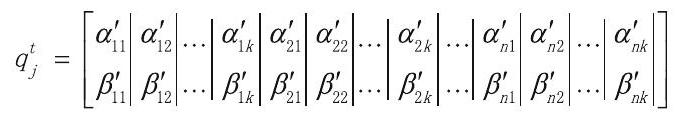
\includegraphics[max width=\textwidth]{2023_06_23_b12b6b8aa353d93821cag-04}
\end{center}

Among them, $\mathrm{q}_{\mathrm{j}}^{\mathrm{t}}$ is the $\mathrm{jt}$ member of the $\mathrm{t}$ generation, and $\mathrm{k}$ is the qubit number used for the components of each independent variable.

Take a 3 bit quantum chromosome as an example to illustrate quantum individuals:

$$
Q=\left[\begin{array}{c|c|c}
1 & \frac{1}{3} & 0 \\
0 & \frac{\sqrt{8}}{3} & 1
\end{array}\right]
$$

This individual contains states: $|000| 001,,|010| 011,,|100| 101,, \mid 110$, and $\mid 111$. The probability is $0,1 / 9,0,8 / 9,0,0,0,00$ (The proportion of the state $|001\rangle$ is $\left.(1)^{2} \times(1 / 3)^{2} \times 1^{2}=1 / 9\right)$. From this example, We can see that $2^{3}=8$ states only need 3 quantum chromosomes to represent, so the quantum chromosome has the characteristics of diversity. As the quantum chromosomes $\left|\alpha_{i}\right|^{2}$ and $\left|\beta_{i}\right|^{2}$ gradually approach 1 or 0 , the quantum chromosomes gradually converge to a single state, the diversity of the population disappears, and the algorithm converges.

\section{Application of Improved Quantum Evolutionary Algorithm in 0-1 Knapsack Problem}
Based on the characteristics of 0-1 knapsack problem, this essay proposes an improved quantum evolutionary algorithm (IQEA) based on dynamic rotation angle catastrophe technology and designs a quantum rotating gate operator which adaptively adjusts the values of rotation angle according to the fitness value and evolution generations. In the process of evolution, the early quantum rotation angle is used to carry out the catastrophic operation of some individuals. The individual and the individual after the catastrophe are evolved in parallel, and the multipath optimization is carried out to improve the parallelism of the algorithm. This can effectively make the population jump out of the current optimal solution, increase the diversity of the population, carry out multi direction search, and maintain the stability of the population, and ensure that the excellent information in the subpopulation will not be lost.

\subsection{Quantum Coding of the 0-1 Knapsack Problem}
In this essay, the 0-1 knapsack problem is quantum coded, and the matrix representation is used to characterize the 0-1 knapsack problem. Each qubit satisfies $\left|\alpha_{i}\right|^{2}+\left|\beta_{i}\right|^{2}=1$ and can be represented by $\left(\begin{array}{c}\alpha_{i} \\ \beta_{i}\end{array}\right)$. After observation, the population is a binary coded 0-1 backpack matrix. Hypothesis that the quantum population size is SizePop and the number of 0-1 knapsack nodes is $\mathrm{n}$, the length of each quantum chromosome is $\mathrm{L}=2 \mathrm{n}$. Then, the coding form of the ith individual in the group $\mathrm{Q}(\mathrm{t})=\left\{\mathrm{q}_{1}^{\mathrm{t}}, \mathrm{q}_{2}^{\mathrm{t}}, \ldots, \mathrm{q}_{\text {sizepop }}^{\mathrm{t}}\right\}$ is:

$$
\mathrm{q}_{i}^{t}=\left(\begin{array}{cccccc}
\alpha_{1} & \alpha_{2} & \ldots & \alpha_{j} & \ldots & \alpha_{n} \\
\beta_{1} & \beta_{2} & & \beta_{j} & & \beta_{n}
\end{array}\right)
$$

In this essay, $\frac{1}{\sqrt{2}}$ is used as the initial of $\alpha_{i}$ and $\beta_{i}$ in the population, which effectively guarantees that all states appear with the same probability.

\subsection{IQEA Algorithm Flow}
Step1: Make $\mathrm{t}=0$, generate the initial population $\mathrm{Q}(\mathrm{t})$ by using the probability quantum chromosome;

Step2: The initial population is measured and the classical chromosomal state $\mathrm{P}(\mathrm{t})$ that solves the 0-1 knapsack problem is obtained;

Step3: Calculate each state fitness value;

Step4: Record the fitness of the best individual;

Step 5: while (Maximum number of iterations or no update generation)

\{

$\mathrm{t++}$

Improved quantum revolving door for updating individual populations;

\{

When the evolution of the population tends to stagnate;

A group of catastrophic technology is initiated by using a certain probability as trigger;

\}

The quantum measurement and decoding of the population $\mathrm{Q}(\mathrm{t})$ is carried out. The state $\mathrm{P}(\mathrm{t})$ is obtained;

The fitness of each state is calculated;

Record the fitness of the best individual.

\}

\subsection{A New Quantum Rotation Gate Operation}
In this IQEA, make the quantum rotation gate $U_{R}(\theta)=\left(\begin{array}{cc}\cos \theta & -\sin \theta \\ \sin \theta & \cos \theta\end{array}\right)$ act on the quantum chromosome to update its gene bit. The quantum rotating gate is a $2 \times 2$ matrix to represent a bit, and the quantum bit is updated by changing the direction and size of the quantum rotation angle. The corresponding operation is [14]:

$$
\left(\begin{array}{c}
\alpha_{i}^{\prime} \\
\beta_{i}^{\prime}
\end{array}\right)=U_{R}(\theta) \cdot\left(\begin{array}{c}
\alpha_{i} \\
\beta_{i}
\end{array}\right)=\left(\begin{array}{cc}
\cos \theta & -\sin \theta \\
\sin \theta & \cos \theta
\end{array}\right) \cdot\left(\begin{array}{c}
\alpha_{i} \\
\beta_{i}
\end{array}\right)
$$

In which $\theta$ is rotation angle, the quantum chromosome $\left(\begin{array}{c}\alpha_{i} \\ \beta_{i}\end{array}\right)$ is transformed into $\left(\begin{array}{l}\alpha_{i}^{\prime} \\ \beta_{i}^{\prime}\end{array}\right)$ after quantum rotation gate operation. The rotation angle $\theta$ and the rotation direction are selected from the Table 1 quantum rotation angle direction and size selection table.

Table 1. Quantum rotation angle direction and size selection table

\begin{center}
\begin{tabular}{l|l|l|l|l|l|l|l}
\hline
$\mathrm{x}_{\mathrm{i}}$ & $\mathrm{b}_{\mathrm{i}}$ & $\mathrm{f}\left(\mathrm{x}_{\mathrm{i}}\right)>\mathrm{f}\left(\mathrm{b}_{\mathrm{i}}\right)$ & $\Delta \theta$ & \multicolumn{4}{|l}{$\mathrm{S}\left(\alpha_{i}, \beta_{i}\right)$} \\
\cline { 4 - 8 }
 &  &  & $\alpha_{i} \beta_{i}>0$ & $\alpha_{i} \beta_{i}<0$ & $\alpha_{i}=0$ & $\alpha_{i}=0$ &  \\
\hline
0 & 0 & $\mathrm{~F}$ & 0 & 0 & 0 & 0 & 0 \\
\hline
0 & 0 & $\mathrm{~T}$ & 0 & 0 & 0 & 0 & 0 \\
\hline
0 & 1 & $\mathrm{~F}$ & 0 & 0 & 0 & 0 & 0 \\
\hline
0 & 1 & $\mathrm{~T}$ & $\delta$ & -1 & 1 & \textbackslash pm 1 & 0 \\
\hline
1 & 0 & $\mathrm{~F}$ & $\delta$ & -1 & 1 & \textbackslash pm 1 & 0 \\
\hline
1 & 0 & $\mathrm{~T}$ & $\delta$ & 1 & -1 & 0 & \textbackslash pm 1 \\
\hline
1 & 1 & $\mathrm{~F}$ & $\delta$ & 1 & -1 & 0 & \textbackslash pm 1 \\
\hline
1 & 1 & $\mathrm{~T}$ & $\delta$ & 1 & -1 & 0 & \textbackslash pm 1 \\
\hline
\end{tabular}
\end{center}

The $\Delta \theta$ value of the quantum rotation angle in the upper table is generally a fixed value, which is fixed by selecting the rotation angle to update the gene location of the quantum chromosome through the look-up table, which can easily lead to the loss of the diversity of the population, thus making the search easy to fall into the local optimal. In this essay, a quantum rotating gate operator is designed for the $0-1$ knapsack problem, which adaptively adjusts the value of the rotation angle according to the fitness value and the evolutionary generations. The concrete realization is as follows: It is assumed that the values of ith bit in the individual $\mathrm{x}$ and the best individual $\mathrm{b}$ after the use of quantum measurements in a population are represented by xi and $b_{\mathrm{i}}$ respectively. The fitness functions $\mathrm{F}(\mathrm{xi})$ and $\mathrm{F}(\mathrm{bi})$ are used to represent individual fitness values, respectively. Combined with Table 1 of this paper, the value of the dynamic quantum rotation angle can be defined by the following formula:

$$
\theta=S \Delta \theta\left(e^{\frac{a b s\left(F\left(x_{i}\right)-F\left(b_{i}\right)\right)}{t}}-1\right)
$$

In which $\Delta \theta$ is an initial rotation angle, the rotation direction of the quantum rotation angle $S$ can be shown in combination with Table 1, and ' $\mathrm{t}$ ' is the current evolutionary generations carried out by the algorithm. The values of the functions $F(x i)$ and $\mathrm{F}$ (bi) change as the evolutionary generation increases. In the course of evolution, the quantum rotation angle is dynamically changed according to the rate of convergence. When the algorithm is in the initial stage of evolution and continuously searches for better solutions, the quantum rotation angle is larger, so that the algorithm can search in a larger range of space. As the evolutionary generations of the algorithm is increasing, the value difference of the optimal solution of the contemporary solution is slowly changing hours, and the quantum rotation angle is becoming smaller and smaller, with the convergence of the algorithm gradually approaching zero.

\subsection{Group Catastrophe Technology}
In the evolution of quantum evolutionary algorithm, the quantum chromosome collapses to a certain direction under the action of the quantum rotation gate adjustment strategy. If the algorithm does not join the mutation operation during the evolution process, when the equivalent sub bit appears in the convergence state, the measured value will be fixed to 0 or 1 . It is difficult to jump out again, and the algorithm is easy to have a prematurity problem. When the algorithm does not change for several generations in the optimal solution, it shows that the algorithm falls into the local optimal value. At this point, catastrophic operation can be carried out on the population, and a greater disturbance will be imposed on the population in the process of evolution, so that it will be separated from the local optimum. When the continuous $\mathrm{N}$ generations are not renewed, the quantum gates are triggered by mutation probability to perform quantum dyeing catastrophic operation.

Because quantum individuals are uncertain in the measurement of decoding, the decoding process may be out of the local optimum, so the catastrophic operation uses the rotation angle in the early stage of evolution to greatly disturb some individuals. Realize the parallel evolution of contemporary superior individuals and postcatastrophe individuals, perform multi-path optimization, and improve the parallelism of the algorithm. This can effectively make the population jump out of the current optimal solution, increase the diversity of the population, conduct multidirectional search, and also maintain the stability of the population, ensuring that the excellent information in the offspring population will not be lost.

\subsection{Quantum Measurement}
The process of quantum measurement is mainly the process of transforming a quantum chromosome into a classical body, making them corresponding to the classical chromosomes, and establishing the corresponding relationship with the solution of the problem. Specific description is: when measuring (or selecting state), it is based on qubit probability amplitude $\left|\alpha_{\mathrm{ij}}\right|^{2}$ (or $\left|\beta_{\mathrm{ij}}\right|^{2}$ ) to select 0 or 1 of the corresponding gene position. The specific method of this paper is: use the random function rand $(0,1)$ to generate a random number $r$, how its value is greater than and if it is greater than the value of $\left|\alpha_{i j}\right|^{2}\left(\right.$ or $\left|\beta_{\mathrm{ij}}\right|^{2}$ ), then generate 0 or 1 , the measurement result is 1 ; otherwise, it takes 0 (or vice versa).

\section{Results Analysis}
In this essay selects the 0-1 knapsack optimization problem with 100 items to carry out experiment. For simplicity, it is recorded as KP100. Each item is encoded in a quantum bit, so the quantum chromosome length is the number of items. In this paper, MATLAB is used to implement the algorithm. The population sizes are set to 10 and 20 respectively. The maximum evolution generations is 500 . The algorithm is solved by traditional EA, QEA and IQEA respectively. Each case runs continuously for 10 times. Then the data of 10 highest fitness values searched 10 times are analyzed statistically. When optimizing the knapsack problem, m denotes the population size, $\mathrm{f}(\mathrm{x})$ denotes the maximum fitness value that is searched for every 10 times. "Best", "Worst" and "Average" represent the maximum fitness values, the minimum fitness values and the average fitness values for the 10 best results found in 10 consecutive experiments respectively. In this essay, all termination conditions for knapsack optimization are the largest evolution generations is 500 . In this essay, the most important index to judge the effect of optimization is "mean", that is, the average fitness of 10 searches.

According to the data in Table 2, the quantum evolution algorithm based on the dynamic rotation angle catastrophe technique has obvious advantages in obtaining the accuracy of the optimal solution. For different initial population sizes, the search ability is different. When the population size is small, the three algorithms do not find the optimal solution in 500 generations. When the population size reaches a certain number, the result of the algorithm is better. Enhanced, IQEA can better find the optimal solution, and the average result is also close to the optimal result, but continue to increase the population size, and does not greatly improve the accuracy of the results.

Table 2. KP100's experimental data table

\begin{center}
\begin{tabular}{l|l|l|l|l}
\hline
$\mathrm{m}$ & $\mathrm{f}(\mathrm{x})$ & EA & QEA & IQEA \\
\hline
\multirow{2}{*}{10} & Best & 3264 & 3938 & 3943 \\
\cline { 2 - 5 }
 & Worst & 3099 & 3776 & 3907 \\
\cline { 2 - 5 }
 & Mean & 3192 & 3878 & 3930 \\
\hline
\multirow{2}{*}{20} & Best & 3342 & 3960 & 3979 \\
\cline { 2 - 5 }
 & Worst & 3176 & 3936 & 3961 \\
\cline { 2 - 5 }
 & Mean & 3245 & 3953 & 3968 \\
\hline
\end{tabular}
\end{center}

Figure 1 is a graph of three algorithms for KP100 with a population of 20. From the convergence graph of Fig. 1, it can be seen that the improved quantum evolution algorithm is more difficult to fall into local optimum and the convergence speed is faster.

\begin{center}
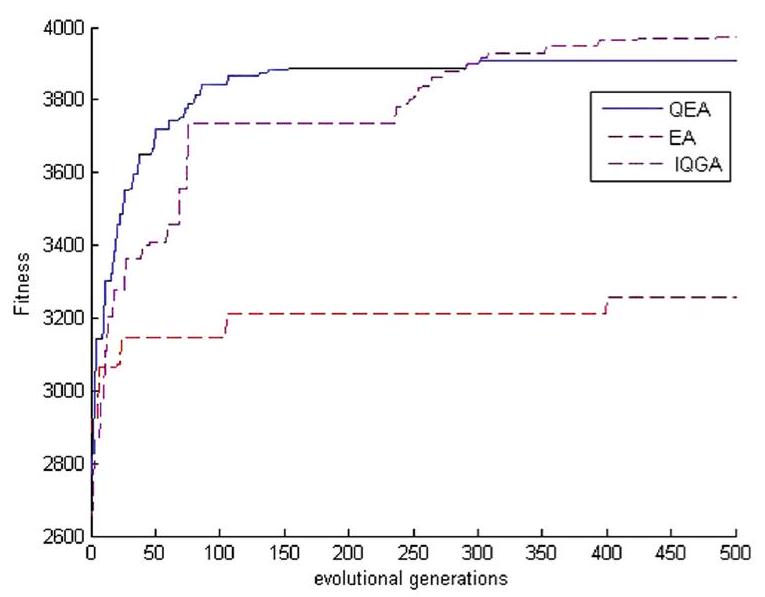
\includegraphics[max width=\textwidth]{2023_06_23_b12b6b8aa353d93821cag-09}
\end{center}

Fig. 1. Comparison of KP100 experiments

\section{Conclusion}
Based on the characteristics of 0-1 knapsack problem, this essay proposes an improved quantum evolutionary algorithm (IQEA) based on dynamic rotation angle catastrophe technology and designs a quantum rotating gate operator which adaptively adjusts the values of rotation angle according to the fitness value and evolution generations. In the process of evolution, the early quantum rotation angle is used to carry out the catastrophic operation of some individuals. The individual and the individual after the catastrophe are evolved in parallel, and the multipath optimization is carried out to improve the parallelism of the algorithm. This can effectively make the population jump out of the current optimal solution, increase the diversity of the population, carry out multi direction search, and maintain the stability of the population, and ensure that the excellent information in the subpopulation will not be lost. The experimental results show that the improved quantum evolution algorithm is better than the evolutionary algorithm and the traditional quantum evolution algorithm in solving the $0-1$ knapsack problem.

\section{References}
\begin{enumerate}
  \item Mathews, G.B.: On the partition of numbers. Lond. Math. Soc. 28, 486-490 (1897)

  \item Wang, X.Z., He, Y.C.: Evolutionary algorithms for knapsack problems. Ruan Jian Xue Bao/J. Softw. 28(1), 1-16 (2017). (in Chinese)

  \item Narayanan, A., Moore, M.: Quantum inspired genetic algorithm. In: IEEE International Conference on Evolutionary Computation, Iscataway, pp. 61-66 (1996)

  \item Han, K.-H., Kim, J.-H.: Genetic quantum algorithm and its application to optimization problem. In: Proceedings of the 2000 IEEE Congress on Evolutionary. IEEE Press, USA, pp. $1354-1360(2000)$ 5. Han, K.-H., Park, K.-H., Lee, C.-H.: Parallel quantum inspired genetic combinatorial optimization problem. In: Proceedings of the 2001 IEEE Congress on Combinatorial Computation algorithm for Evolutionary Computation. IEEE Press, USA, pp. 1422-1429 $(2001)$

  \item Han, K.-H., Kim, J.-H.: On the analysis of the quantum-inspired evolutionary algorithm with a single individual. In: Proceedings of the 2006 IEEE Congress on Evolutionary Computation. IEEE Press, USA, pp. 2622-2629 (2006)

  \item Yang, J.A., et al.: Multi-cosmic parallel quantum genetic algorithm. Chin. J. Electron. 32(6), 923-928 (2004)

  \item Zhang, G.X., et al.: A novel quantum genetic algorithm and its application. ACTA Electr. Sin. 32(3), 476-479 (2004)

  \item Chen, H., et al.: Chaos updating rotated gates quantum-inspired genetic algorithm. In: Proceedings of the International Conference on Communications, Circuits and systems, vol. 2, pp. 1108-1112 (2004)

  \item Ling, W., et al.: Hybrid numerical optimization genetic algorithm based on quantum computing for and parameter estimation. Appl. Math. Comput. 171, 1141-1156 (2005)

  \item Li, S., et al.: Quantum genetic algorithm based on real coding and gradient of objective function. J. Harbin Univ. Technol. 38(8), 1216-1218, 1223 (2006)

  \item Liang, X.: Research on the application of evolutionary algorithms and quantum computing in optimization problems. China University of Science and Technology (2012). \href{https://doi}{https://doi}. org/10.7666/d.y 2125828

  \item Bhatia, A.K., Basu, S.K.: Tackling 0/1 knapsack problem with gene induction. Soft. Comput. 8(1), 1-9 (2003)

  \item Li, J.L., et al.: A new quantum rotation angle of quantum-inspired evolutionary algorithm for TSP. Int. J. High Perform. Syst. Arch. 7(4), 223-230 (2017)

\end{enumerate}

\end{document}